\documentclass{article}

\usepackage[utf8]{inputenc}
\usepackage{amsmath}

\usepackage{tikz}

\begin{document}

    \title{}
    \author{}
    \date{}

    Based on https://mattmazur.com/2015/03/17/a-step-by-step-backpropagation-example/

    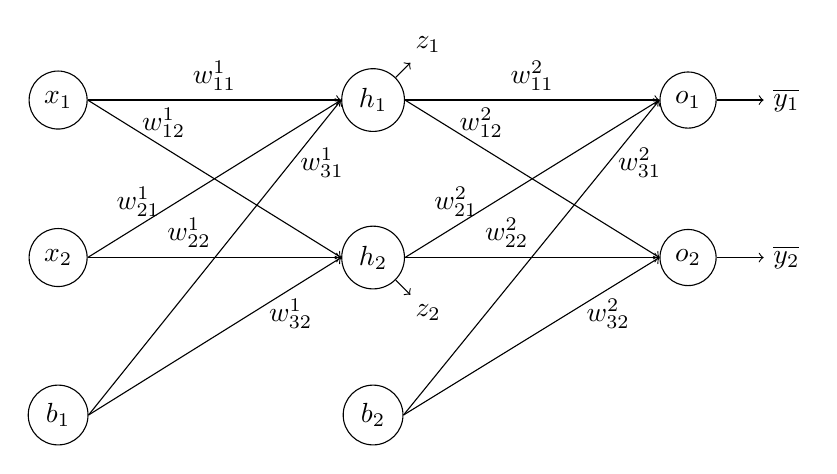
\begin{tikzpicture}
    \tikzstyle{neuron}=[circle,draw=black,minimum size=17pt]

    \node[neuron] (x1) {$x_1$};
    \node[neuron] (x2) at (0, -2) {$x_2$};
    \node[neuron] (b1) at (0, -4) {$b_1$};

    \node[neuron] (h1) at (4, 0)  {$h_1$};
    \node[neuron] (h2) at (4, -2) {$h_2$};
    \node[neuron] (b2) at (4, -4) {$b_2$};

    \node[neuron] (o1) at (8, 0)  {$o_1$};
    \node[neuron] (o2) at (8, -2) {$o_2$};

    \draw[->] (x1.east) -- (h1.west) node[midway,above] {$w_{11}^1$};
    \draw[->] (x1.east) -- (h2.west) node[pos=0.3,above] {$w_{12}^1$};
    \draw[->] (x2.east) -- (h1.west) node[pos=0.2,above] {$w_{21}^1$};
    \draw[->] (x2.east) -- (h2.west) node[pos=0.4,above] {$w_{22}^1$};
    \draw[->] (b1.east) -- (h1.west) node[pos=0.8,right] {$w_{31}^1$};
    \draw[->] (b1.east) -- (h2.west) node[pos=0.8,below] {$w_{32}^1$};

    \draw[->] (h1.east) -- (o1.west) node[midway,above] {$w_{11}^2$};
    \draw[->] (h1.east) -- (o2.west) node[pos=0.3,above] {$w_{12}^2$};
    \draw[->] (h2.east) -- (o1.west) node[pos=0.2,above] {$w_{21}^2$};
    \draw[->] (h2.east) -- (o2.west) node[pos=0.4,above] {$w_{22}^2$};
    \draw[->] (b2.east) -- (o1.west) node[pos=0.8,right] {$w_{31}^2$};
    \draw[->] (b2.east) -- (o2.west) node[pos=0.8,below] {$w_{32}^2$};

    \node at (4.7, 0.7) (z1) {$z_1$};
    \node at (4.7, -2.7) (z2) {$z_2$};

    \draw[->] (h1) -- (z1);
    \draw[->] (h2) -- (z2);

    \node at (9.25, 0) (y1) {$\overline{y_1}$};
    \node at (9.25, -2) (y2) {$\overline{y_2}$};

    \draw[->] (o1) -- (y1);
    \draw[->] (o2) -- (y2);
\end{tikzpicture}


    \begin{equation}
        E = \frac{1}{2} \sum_{i}{(y_i - \overline{y_i})^2} = 
        \frac{1}{2} \left[ (y_1 - \overline{y_1})^2 + (y_2 - \overline{y_2})^2 \right]
    \end{equation}

    \begin{equation*}
        \frac{\partial E}{\partial y_1} = \overline{y_1} - y_1
        \qquad % horizontal space
        \frac{\partial E}{\partial y_2} = \overline{y_2} - y_2
    \end{equation*}

    \begin{equation}
        \overline{y_1} = \frac{1}{1+ e^{-o_1}}
        \qquad % horizontal space
        \overline{y_2} = \frac{1}{1+ e^{-o_2}}
    \end{equation}

    \begin{equation*}
        \frac{\partial \overline{y_1}}{\partial o_1} = \overline{y_1} (1 - \overline{y_1})
        \qquad % horizontal space
        \frac{\partial \overline{y_2}}{\partial o_2} = \overline{y_2} (1 - \overline{y_2})
    \end{equation*}

    \begin{equation*}
        \frac{\partial E}{\partial o_1} = 
        \frac{\partial E}{\partial \overline{y_1}} \frac{\partial \overline{y_1}}{\partial o_1}
        \qquad % horizontal space
        \frac{\partial E}{\partial o_2} =
        \frac{\partial E}{\partial \overline{y_2}} \frac{\partial \overline{y_2}}{\partial o_2}
    \end{equation*}

    \begin{equation}
        o_1 =  z_1 w_{11}^2 + z_2 w_{21}^2 + b_2 w_{31}^2
        \qquad % horizontal space
        o_2 =  z_1 w_{12}^2 + z_2 w_{22}^2 + b_2 w_{32}^2
    \end{equation}

    \begin{equation*}
        \frac{\partial o_1}{\partial w_{11}^2} = z_1
        \qquad % horizontal space
        \frac{\partial o_1}{\partial w_{21}^2} = z_2
        \qquad % horizontal space
        \frac{\partial o_1}{\partial z_1} = w_{11}^2
        \qquad % horizontal space
        \frac{\partial o_1}{\partial z_2} = w_{21}^2
    \end{equation*}

    \begin{equation*}
        \frac{\partial o_2}{\partial w_{12}^2} = z_1
        \qquad % horizontal space
        \frac{\partial o_2}{\partial w_{22}^2} = z_2
        \qquad % horizontal space
        \frac{\partial o_2}{\partial z_1} = w_{12}^2
        \qquad % horizontal space
        \frac{\partial o_2}{\partial z_2} = w_{22}^2
    \end{equation*}

    \begin{equation*}
        \frac{\partial E}{\partial z_1} = 
        \frac{\partial E}{\partial o_1} \frac{\partial o_1}{\partial z_1} +
        \frac{\partial E}{\partial o_2} \frac{\partial o_2}{\partial z_1}
    \end{equation*}

    \begin{equation*}
        \frac{\partial E}{\partial z_2} = 
        \frac{\partial E}{\partial o_1} \frac{\partial o_1}{\partial z_2} +
        \frac{\partial E}{\partial o_2} \frac{\partial o_2}{\partial z_2}
    \end{equation*}

    \begin{equation}
        z_1 = \frac{1}{1+ e^{-h_1}} 
        \qquad % horizontal space
        z_2 = \frac{1}{1+ e^{-h_2}} 
    \end{equation}

    \begin{equation*}
        \frac{\partial z_1}{\partial h_1} = z_1 (1 - z_1)
        \qquad % horizontal space
        \frac{\partial z_2}{\partial h_2} = z_2 (1 - z_2)
    \end{equation*}

    \begin{equation}
        h_1 =  x_1 w_{11}^1 + x_2 w_{21}^1 + b_1 w_{31}^1
        \qquad % horizontal space
        h_2 =  x_1 w_{12}^1 + x_2 w_{22}^1 + b_1 w_{32}^1
    \end{equation}

    \begin{equation*}
        \frac{\partial h_1}{\partial w_{11}^1} = x_1
        \qquad % horizontal space
        \frac{\partial h_1}{\partial w_{21}^1} = x_2
    \end{equation*}

    \begin{equation*}
        \frac{\partial h_2}{\partial w_{12}^1} = x_1
        \qquad % horizontal space
        \frac{\partial h_2}{\partial w_{22}^1} = x_2
    \end{equation*}


\end{document}
